\documentclass[conference, 11pt]{IEEEtran}
\IEEEoverridecommandlockouts
% The preceding line is only needed to identify funding in the first footnote. If that is unneeded, please comment it out.
\usepackage{cite}
\usepackage{amsmath,amssymb,amsfonts}
\usepackage{algorithmic}
\usepackage{graphicx}
\usepackage{textcomp}
\usepackage{xcolor}
\usepackage{hyperref}
\hypersetup{
colorlinks=true,
linkcolor=blue,
filecolor=blue,
citecolor=black,      
urlcolor=cyan,
}
\def\BibTeX{{\rm B\kern-.05em{\sc i\kern-.025em b}\kern-.08em
    T\kern-.1667em\lower.7ex\hbox{E}\kern-.125emX}}
\begin{document}

\bstctlcite{IEEEexample:BSTcontrol}

\makeatletter
\newcommand{\linebreakand}{%
  \end{@IEEEauthorhalign}
  \hfill\mbox{}\par
  \mbox{}\hfill\begin{@IEEEauthorhalign}
}
\makeatother

\title{SAIRA: Student Affairs AI Response Assistant}

\author{\IEEEauthorblockN{Vladimir Makharev}
\IEEEauthorblockA{\textit{Innopolis University}\\
Innopolis, Russia \\
\href{mailto:v.makharev@innopolis.university}{v.makharev@innopolis.university}}
\and
\IEEEauthorblockN{Artem Batalov}
\IEEEauthorblockA{\textit{Innopolis University}\\
Innopolis, Russia \\
\href{a.batalov@innopolis.university}{a.batalov@innopolis.university}}
\linebreakand
\IEEEauthorblockN{Danil Andreev}
\IEEEauthorblockA{\textit{Innopolis University}\\
Innopolis, Russia \\
\href{d.andreev@innopolis.university}{d.andreev@innopolis.university}}
\and
\IEEEauthorblockN{Evgenii Evlampev}
\IEEEauthorblockA{\textit{Innopolis University}\\
Innopolis, Russia \\
\href{e.evlampev@innopolis.university}{e.evlampev@innopolis.university}}
}

\maketitle

\begin{abstract}
This project implement an AI-driven support system for Innopolis University using Large Language Models (LLMs), specifically focusing on autonomously handling rudimentary student queries. The study integrates Transformer-based LLMs with Retrieval Augmented Generation (RAG) and LlamaIndex to enhance the university's existing support platform. By employing parsers for data aggregation from diverse university websites and utilizing a Vector Store index with BAAI General Embedding for indexing, the system significantly improves in handling basic inquiries. Experimental results, particularly with models like 'simple-mistral-instruct-7b-emb-large-default', demonstrate a notable increase in efficiency, as measured by BLEU, ROUGE, and METEOR metrics. This approach not only reduces the workload on customer support staff but also offers quicker and more accurate responses to students, showcasing the potential of AI in transforming educational support systems.

GitHub link to the project: \href{https://github.com/kilimanj4r0/SAIRA}{https://github.com/kilimanj4r0/SAIRA}
\end{abstract}

\begin{IEEEkeywords}
LLM, knowledge base, chat-bot, retrieval augmented generation
\end{IEEEkeywords}

\section{Introduction}

\begin{figure}[h]
\centering

\includegraphics[width=0.4\linewidth]{saira.png}
\caption{Project Logo}
\end{figure}

Over time, knowledge base systems have significantly contributed to the efficiency of organizational processes. A notable example of such advancement is the integration of AI in customer support, particularly in self-service modalities.

Innopolis University utilizes a support system, accessible at \href{http://omnidesk.ru}{omnidesk.ru}, specifically designed to aid students. This platform is tailored to streamline customer service interactions and elevate the overall support experience. However, it currently lacks the functionality to autonomously address basic inquiries from students.

The Student Affairs Office reports that approximately $20\%$ of all queries submitted to this system are rudimentary and could be resolved autonomously, utilizing the University's knowledge base.

This observation indicates a significant opportunity for enhancing the system's efficiency. By integrating an AI-driven response mechanism, capable of leveraging the existing University knowledge base, the system could autonomously handle these rudimentary queries. Such an upgrade would not only reduce the workload on customer support staff but also expedite response times for students, thereby improving the overall user experience.

\section{Related work}
The Transformer Architecture \cite{attention_is_all_you_need} has improved the state-of-the-art in various sequence modeling tasks. Transformer-based Large Language Models (LLM), such as GPT \cite{gpt}, LLaMA \cite{llama}, and Mistral \cite{mistral}, with billions of parameters, have displayed near-human or sometimes even superhuman performance on specific tasks. The capability to process and generate coherent and contextually relevant text has led to their widespread adoption.

One of the possible applications of LLMs is as domain-specific knowledge base assistants, where models excel in providing tailored information and insights across various specialized fields. In this role, LLMs can interpret and respond to intricate queries in a conversational manner, making them particularly useful as support assistants. Nevertheless, their proficiency in accessing and meticulously managing knowledge is somewhat restricted. Therefore, in tasks that demand substantial knowledge, their effectiveness is not as advanced as task-specific systems. Furthermore, the challenges of tracing the origins of their decisions and keeping their global knowledge up-to-date are still areas of ongoing research.

\subsection{Fine-tuning LLM}
Fine-tuning adapts the LLM's weights to custom domains and tasks.

Data scientists feed the model a collection of prompts and expected responses. The model learns the gaps between what it currently produces and what the training pipeline expected and adjusts its \emph{attention} to specific features and patterns.

However, fine-tuning requires a large amount of labeled data, which may be scarce, noisy, or expensive to obtain. It also requires significant computational resources, which could present a significant hurdle, so it is difficult to fine-tune new model regularly on new data.

\subsection{Retrieval Augmented Generation (RAG)}

\begin{figure}[h]
\centering
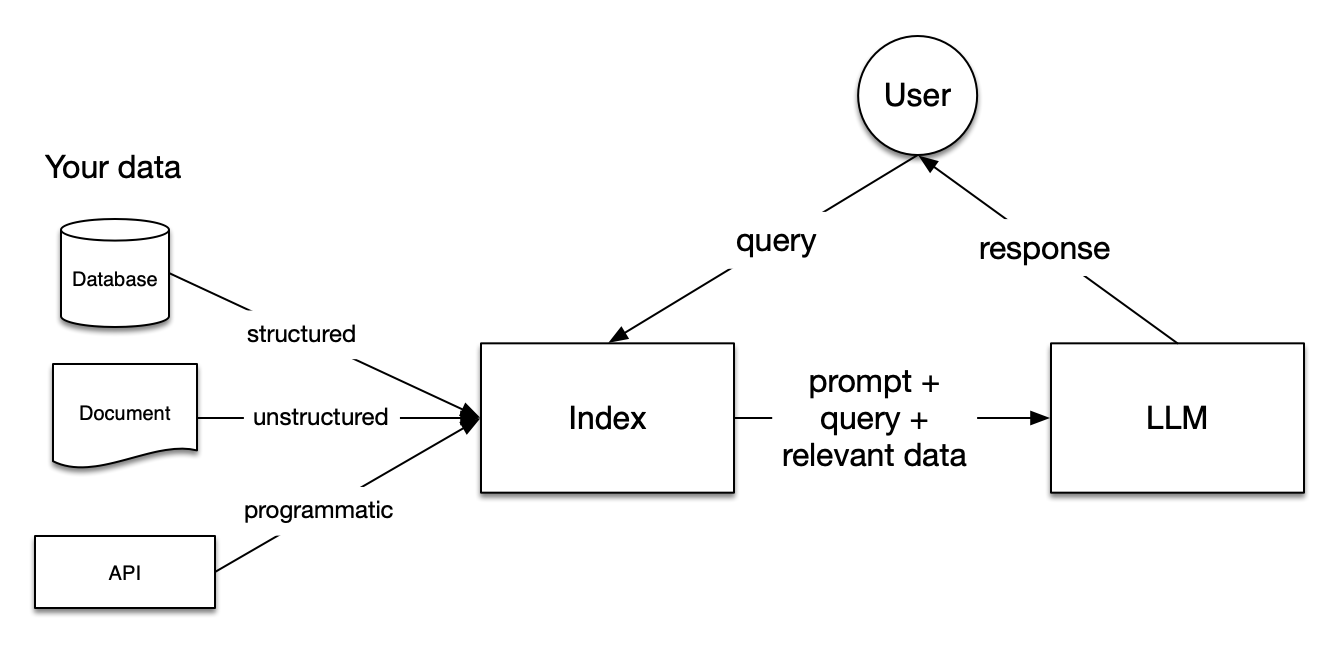
\includegraphics[width=1.0\linewidth]{basic_rag.png}
\caption{Overview of RAG approach \cite{llamaindex_rag}}
\end{figure}

Retrieval Augmented Generation (RAG) \cite{rag} inserts an additional step between users' requests and the generative model. In this step, the pipeline finds information relevant to the user's request and injects it as context. The data is loaded and prepared for queries or ``indexed''. User queries act on the index, which filters your data down to the most relevant context. This context and your query then go to the LLM along with a prompt, and the LLM provides a response. This information could come from:
\begin{itemize}
    \item A vector database such as FAISS \cite{faiss} or Pinecone;
    \item Unstructured documents;
    \item Traditional databases such as SQL or MongoDB;
    \item APIs such as those for Google Maps or IMDB;
    \item A search engine such as Google or Bing.
\end{itemize}

As stated in \cite{rag}, human evaluators were provided with a topic and given two questions in the style of Jeopardy that the topic would respond to. The system inquired which question they deemed more based on facts. Comparatively, the responses from the model improved with RAG were judged as factual $54.4\%$ of the time, in contrast to only $18.8\%$ for the model without RAG enhancement.


\section{Methodology}

\subsection{Information Retrieval}

We have aggregated a catalog of university websites speculated to encompass valuable information. For detailed listings, please consult Table \ref{tab:university_websites}, which outlines these relevant sources.

The data from websites is gathered through parsers. Utilizing parsers enables the automation of data collection, updates, and formatting, significantly contributing to the accuracy of responses generated by Large Language Model (LLM). All parsers are scripted in Python and employ auxiliary packages to extract and format primary information from the websites.

Due to the disparate formats in which information is presented across various websites, distinct packages were employed for different sites. For parsing \href{https://eduwiki.innopolis.university/}{eduwiki.innopolis.university} and \href{https://campuslife.innopolis.ru/}{campuslife.innopolis.ru}, the \texttt{markdownify} package was utilized to convert HTML pages into markdown format. Additionally, \textit{readability} was used for \href{https://campuslife.innopolis.ru/}{campuslife.innopolis.ru} to extract key information from the page, given its abundance of navigational elements and news posts.

\subsection{RAG + LlamaIndex}
There are five key stages within RAG.
\subsubsection{Loading stage}
The loading is getting the data from retrieved files. 

We use \texttt{SimpleDirectoryReader} for loading all our data to the pipeline in a LlamaIndex's \texttt{Document} container, then using \texttt{Node} to represent a ``chunk'' of a source \texttt{Document}.

\subsubsection{Indexing stage}
The indexing is creating a data structure that allows for querying the data. For LLMs this often means creating vector embeddings.

\begin{figure}[h]
\centering
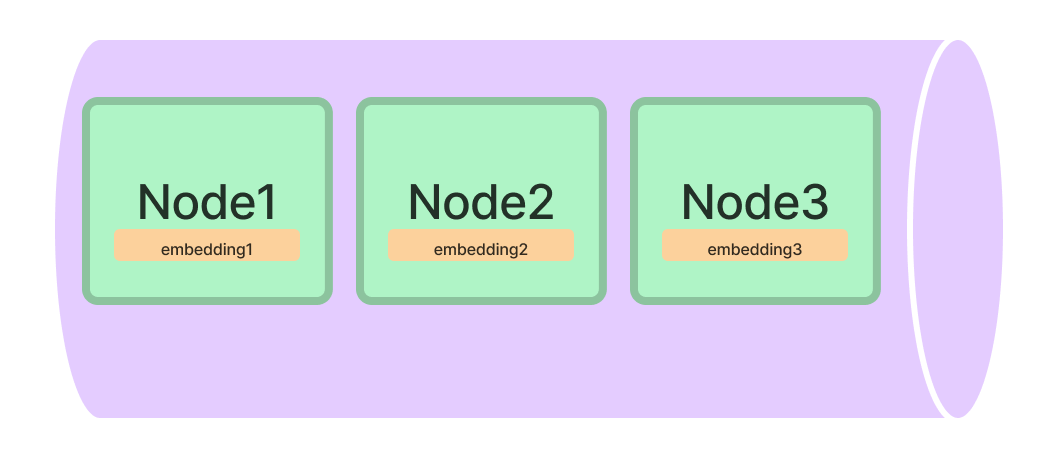
\includegraphics[width=0.8\linewidth]{vector_store.png}
\caption{Vector Store index}
\label{fig:vector_store}
\end{figure}

For our system we use Vector Store index (Fig. \ref{fig:vector_store}). This type index stores each Node and a corresponding embedding.

As embedding model we use BAAI General Embedding \cite{bge}, because according to Massive Text Embedding Benchmark (MTEB) Leaderboard \cite{mteb}, it is a SOTA in retrieval tasks, and it is a fully compatible with LlamaIndex. We also tried to use e5 models family, but there was errors while working with LlamaIndex.

\subsubsection{Storing stage}
Storing the index, as well as other metadata, to avoid having to re-index it.

By default, LlamaIndex's Vector Store index uses a in-memory \texttt{SimpleVectorStore} that’s initialized as part of the default storage context. We also tried to use Chroma vector store, but it worked bad in quering stage, and we have settled on using \texttt{SimpleVectorStore}.

\subsubsection{Querying stage}
There are many ways you can utilize LLMs and LlamaIndex data structures to query, including sub-queries, multi-step queries and hybrid strategies.

\begin{figure}[h]
\centering
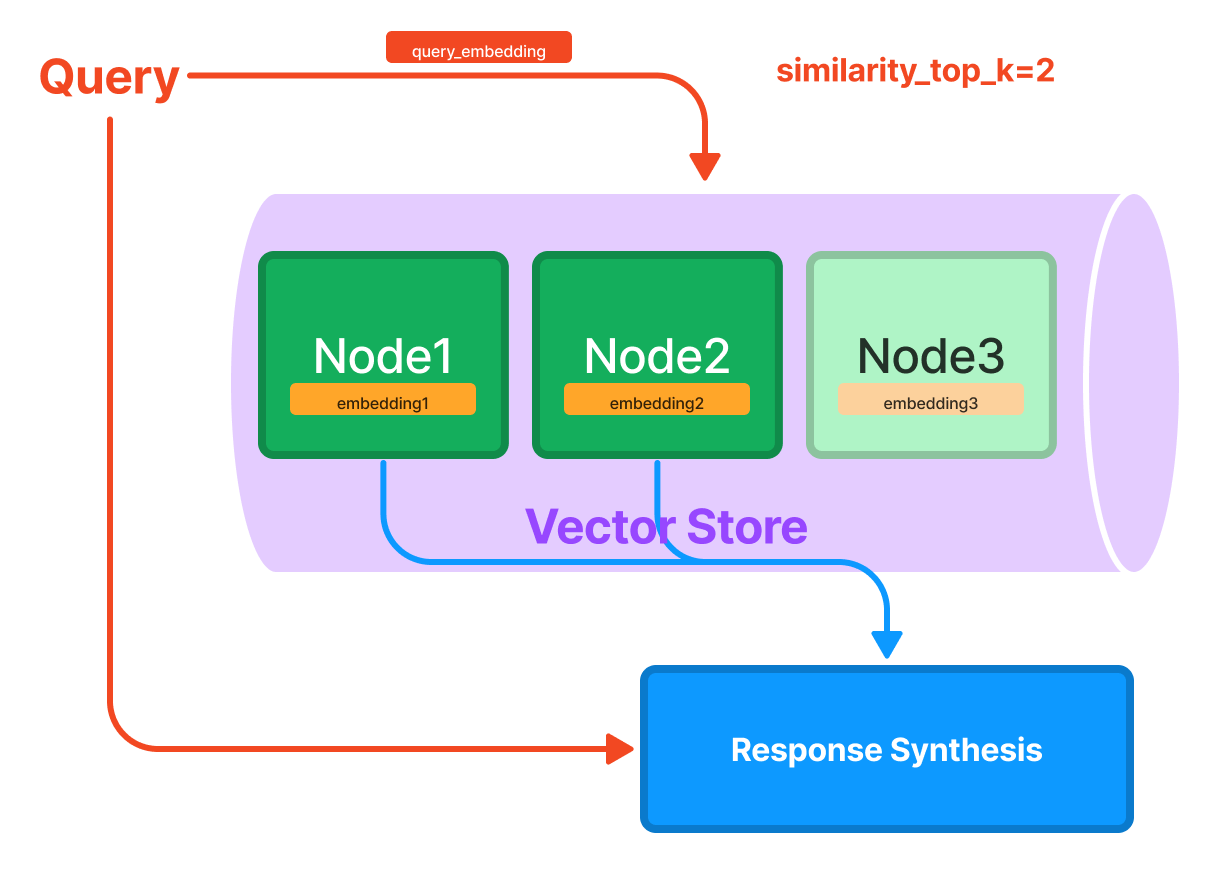
\includegraphics[width=0.8\linewidth]{vector_store_query.png}
\caption{Vector Store index query}
\label{fig:vector_store}
\end{figure}

We tried 2 response modes here, and more similar for us is \texttt{compact}, because \texttt{tree\_summarize} often confuse many node results. More information are available in \ref{experiments} section.

\section{Experiments}
\label{experiments}

In pursuit of identifying the optimal model configuration for our system, an extensive grid search methodology was employed, systematically exploring various combinations of models, vector stores, embedding models, and retriever response modes. The evaluated models encompassed a selection of LLAMA 2 13B, MISTRAL 7B, and ORCA 2 13B, each representing distinct architectures and capacities. Diversified vector stores including SimpleVectorStore and ChromaDB were investigated to discern their impact on system performance. Furthermore, embedding models such as BAAI/bge-small-en and BAAI/bge-large-en-v1.5 were scrutinized for their efficacy in generating embeddings suitable for our task. In tandem, retriever response modes, specifically Tree Summarize and Compact, were tested to appraise their influence on the overall retrieval quality. These experiments were meticulously designed and executed to discern the most optimal combination of components, aiming to enhance the system's performance and effectiveness in handling information retrieval and response generation tasks.

\section{Evaluation}
To evaluate the performance of our system, we employed a combination of automated metrics and human assessments. Specifically, we utilized three widely recognized automated metrics: BLEU (Bilingual Evaluation Understudy), METEOR (Metric for Evaluation of Translation with Explicit ORdering), and ROUGE (Recall-Oriented Understudy for Gisting Evaluation). These metrics were calculated for each response generated by our system to provide a quantifiable measure of its effectiveness in generating relevant and coherent answers.

In addition to these automated evaluations, we also conducted a human evaluation process. This step was crucial for obtaining qualitative feedback on the system's performance. During this phase, evaluators manually reviewed a set of specific samples, allowing us to fine-tune our Retrieval-Augmented Generation (RAG) setup based on their insights. This human-centric approach helped ensure that the system's outputs were not only statistically sound according to the automated metrics but also practically useful and contextually appropriate according to human judgment.

The evaluation process covered a test set consisting of 55 manually crafted question-and-answer pairs. These pairs were specifically designed to rigorously test the system across a variety of topics. To obtain a comprehensive overview of the system's performance, we averaged the scores from each automated metric across all topics in the test set. This approach allowed us to capture a broad and balanced view of the system's capabilities and areas for improvement.

By integrating both automated and human evaluations, we achieved a robust assessment of our system, balancing quantitative precision with qualitative insights. This methodology ensured a thorough and nuanced understanding of the system's strengths and weaknesses.

\section{Analysis}

The table (Table II) presents an exhaustive evaluation of various models across different performance metrics, encompassing Average BLEU, Average ROUGE, and Average METEOR scores. The models were trained and assessed under diverse configurations, delineated by specific vector stores, model architectures (LLAMA 2 13B, MISTRAL 7B, ORCA 2 13B), embedding models, and response modes (default and summarize). Among the evaluated configurations, notable distinctions in performance metrics were observed. Notably, the configuration utilizing the SimpleVectorStore with the MISTRAL 7B architecture and an embedding model of larger dimensions (simple-mistral-instruct-7b-emb-large-default) demonstrated superior performance, yielding the highest Average BLEU, Average ROUGE, and Average METEOR scores of 0.1709, 0.4163, and 0.5018, respectively. Conversely, configurations employing the 'summarize' response mode exhibited comparatively lower scores across all metrics, suggesting potential limitations in summarization-based retrieval methods within the context of this evaluation. These findings underscore the significance of parameter configuration and choice of models, highlighting the notable influence on performance metrics, thereby warranting a meticulous consideration of these factors in optimizing the system's effectiveness for generating accurate and coherent responses.

\section{Conclusion}

The integration of AI-driven response mechanisms, particularly leveraging Large Language Models (LLMs), into Innopolis University's support system presents a transformative opportunity to enhance efficiency and user experience. This project demonstrates that Transformer-based LLMs, fine-tuned and augmented with Retrieval Augmented Generation (RAG) and LlamaIndex, can autonomously handle a significant portion of rudimentary queries within a university setting.

Our approach combined the strengths of different models, embedding techniques, and vector stores to create an effective knowledge base assistant. The use of parsers for data aggregation from university websites, and the implementation of a Vector Store index with BAAI General Embedding for indexing, played a crucial role in the successful application of this technology.

The experiments conducted provided valuable insights into the optimal configuration of models and tools. Pipelines such as 'simple-mistral-instruct-7b-emb-large-default' demonstrated superior performance in terms of BLEU, ROUGE, and METEOR metrics, highlighting the importance of choosing the right combination of tools and techniques.

In conclusion, this project underscores the potential of AI and LLMs in revolutionizing customer support systems in educational institutions. By autonomously addressing basic inquiries, the system not only alleviates the workload of support staff but also ensures timely and accurate responses to students. The continuous development and refinement of such systems are essential for keeping pace with the evolving demands of the educational sector and the broader field of AI-driven customer support solutions.

\section{Future Work}

As we continue to enhance the capabilities of our AI assistant tailored for answering student queries, several avenues for future development have been identified. 

One significant expansion involves the incorporation of (scanned) document parsing, enabling the system to extract information from various document formats to enrich its knowledge base. Additionally, accommodating both English and Russian documents, particularly in scenarios where questions and answers are in English within Russian documents, poses an interesting challenge. This could potentially involve leveraging multilingual models or integrating translation mechanisms within the pipeline to ensure seamless comprehension and response generation. 

These proposed enhancements aim to broaden the AI assistant's scope and improve its efficiency in handling diverse linguistic and informational contexts, thereby augmenting its utility for our users.

We are planning to implement an AI assistant into Innopolis University's current support system, a strategic move aimed at enhancing the efficiency of the platform.

% --------------------------------------------------------------------

\bibliographystyle{IEEEtran}
\bibliography{references}

\clearpage
\onecolumn
\appendices
\section{Tables}

\begin{table*}[h] % Use t, b, or h as per your preference for table positioning
\caption{List of University Websites with Data}
\centering
\begin{tabular}{|l|l|l|}
\hline
\textbf{Website} & \textbf{Data} & \textbf{Link} \\
\hline
University & General Information & \url{https://innopolis.university/} \\
EduWiki & Information on educational programs & \url{https://eduwiki.innopolis.university/} \\
Campus & Information about campus life & \url{https://campuslife.innopolis.ru/} \\
Hotel & Support for accommodation-related queries & \url{https://hotel.innopolis.university/} \\
Sport & Sports for students & \url{https://sport.innopolis.university/} \\
InnoHassle & Schedules & \url{https://innohassle.ru/schedule} \\
\hline
\end{tabular}
\label{tab:university_websites}
\end{table*}

\begin{table}[h]
\caption{Model Metrics}
\centering
\begin{tabular}{|l|c|c|c|}
\hline
\textbf{Model} & \textbf{Average BLEU} & \textbf{Average ROUGE} & \textbf{Average METEOR} \\
\hline
chromadb-llama2-13b-emb-base-default & 0.0371 & 0.1500 & 0.2775 \\
chromadb-llama2-13b-emb-base-summarize & 0.0211 & 0.1121 & 0.2258 \\
chromadb-mistral-instruct-7b-emb-base-default & 0.0640 & 0.2042 & 0.2795 \\
chromadb-mistral-instruct-7b-emb-base-summarize & 0.0222 & 0.1285 & 0.2212 \\
chromadb-orca2-13b-emb-base-default & 0.0271 & 0.1056 & 0.2246 \\
chromadb-orca2-13b-emb-base-summarize & 0.0195 & 0.1017 & 0.2202 \\
simple-mistral-instruct-7b-emb-large-default & \textbf{0.1709} & \textbf{0.4163} & \textbf{0.5018} \\
simple-mistral-instruct-7b-emb-large-summarize & 0.0547 & 0.2094 & 0.3088 \\
simple-orca2-13b-emb-base-default & 0.0511 & 0.1747 & 0.3314 \\
simple-orca2-13b-emb-base-summarize & 0.0379 & 0.1427 & 0.2693 \\
\hline
\end{tabular}
\label{tab:model_metrics_sorted_updated}
\end{table}

\end{document}
